% Fig. 1: the three decisions of JIT-Repair. Compile: pdflatex fig1_method.tex  (190 mm wide)
\documentclass[tikz,border=0pt]{standalone}
\usepackage[T1]{fontenc}
\usepackage{tgheros}
\renewcommand{\familydefault}{\sfdefault}
\usepackage{sansmath}
\usetikzlibrary{arrows.meta,positioning,calc,shapes.geometric,fit,backgrounds}
\definecolor{gated}{HTML}{2A78D6}
\definecolor{uniform}{HTML}{EB6834}
\definecolor{revise}{HTML}{1BAF7A}
\definecolor{ref}{HTML}{6B6A66}
\definecolor{ink}{HTML}{1A1A19}
\definecolor{ink2}{HTML}{52514E}
\definecolor{wash}{HTML}{EEF4FC}
\definecolor{rule}{HTML}{D9D8D3}
\begin{document}
\sansmath\hyphenpenalty=10000\exhyphenpenalty=10000
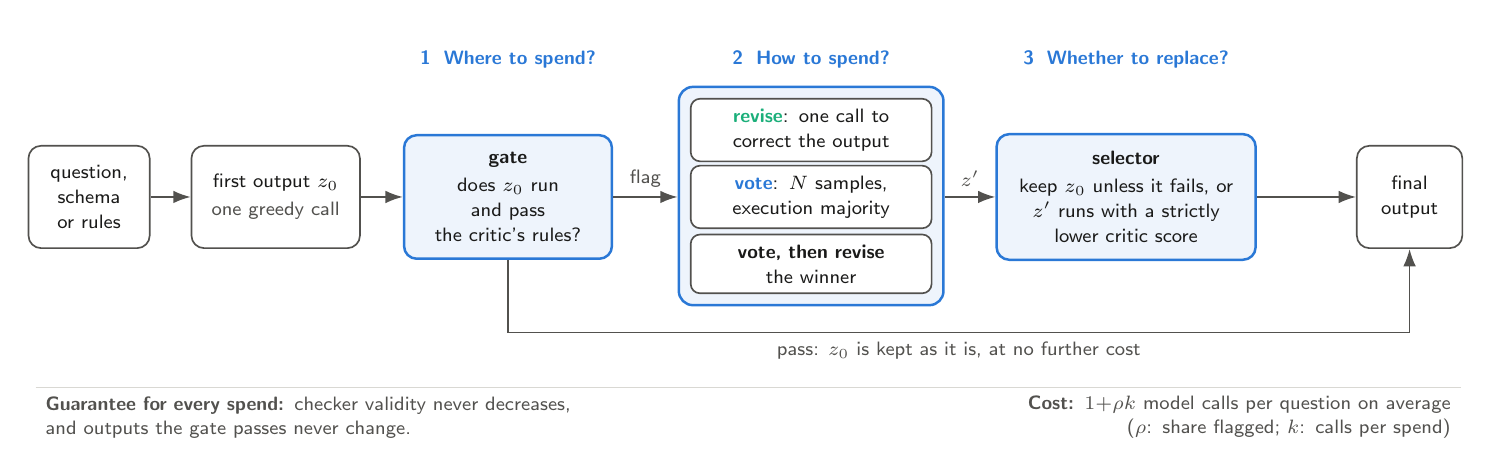
\begin{tikzpicture}[
  font=\fontsize{7.5}{9}\selectfont, line width=0.6pt, >={Latex[length=2.2mm,width=1.6mm]},
  box/.style={draw=ink2, rounded corners=1.6mm, align=center, inner sep=2.2mm, fill=white, text=ink},
  dec/.style={draw=gated, line width=0.9pt, rounded corners=1.6mm, align=center, inner sep=2.2mm, fill=wash, text=ink},
  sp/.style={draw=ink2, rounded corners=1.2mm, align=center, inner sep=1.3mm, fill=white, text=ink, text width=28mm},
  lab/.style={font=\fontsize{7}{8.5}\selectfont\bfseries, text=gated},
  note/.style={font=\fontsize{7}{8.5}\selectfont, text=ink2, align=center},
  arr/.style={->, draw=ink2},
]
% fixed width: 190 mm
\path[use as bounding box] (0,-3.05) rectangle (18.3,2.25);

\node[box, minimum height=13mm, text width=11mm] (x) at (0.78,0.1) {question,\\schema\\or rules};
\node[box, minimum height=13mm, text width=17mm] (z0) at (3.15,0.1) {first output $z_0$\\[1pt]\textcolor{ink2}{one greedy call}};
\node[dec, minimum height=13mm, text width=22mm] (gate) at (6.1,0.1) {\textbf{gate}\\[1pt]does $z_0$ run and pass\\the critic's rules?};
\node[sp] (rev) at (9.95,0.95) {\textcolor{revise}{\textbf{revise}}: one call to\\correct the output};
\node[sp] (vote) at (9.95,0.1) {\textcolor{gated}{\textbf{vote}}: $N$ samples,\\execution majority};
\node[sp] (both) at (9.95,-0.75) {\textbf{vote, then revise}\\the winner};
\begin{scope}[on background layer]
\node[draw=gated, line width=0.9pt, rounded corners=1.8mm, fill=wash, fit=(rev)(vote)(both), inner sep=1.4mm] (spend) {};
\end{scope}
\node[dec, minimum height=13mm, text width=28.5mm] (sel) at (13.95,0.1) {\textbf{selector}\\[1pt]keep $z_0$ unless it fails, or\\$z'$ runs with a strictly\\lower critic score};
\node[box, minimum height=13mm, text width=9mm] (out) at (17.55,0.1) {final\\output};
% stage labels
\node[lab] at (gate.north |- 0,1.85) {1 \;Where to spend?};
\node[lab] at (spend.north |- 0,1.85) {2 \;How to spend?};
\node[lab] at (sel.north |- 0,1.85) {3 \;Whether to replace?};
% arrows
\draw[arr] (x) -- (z0);
\draw[arr] (z0) -- (gate);
\draw[arr] (gate.east) -- node[above, note, pos=0.5] {flag} (spend.west |- gate.east);
\draw[arr] (spend.east |- sel.west) -- node[above, note] {$z'$} (sel.west);
\draw[arr] (sel) -- (out);
% pass path
\draw[arr] (gate.south) -- (gate.south |- 0,-1.62) -- node[below, note, pos=0.5] {pass: $z_0$ is kept as it is, at no further cost} (out.south |- 0,-1.62) -- (out.south);
% footer
\draw[rule, line width=0.5pt] (0.1,-2.32) -- (18.2,-2.32);
\node[note, anchor=west, text width=100mm, align=left] at (0.1,-2.7) {\textbf{Guarantee for every spend:} checker validity never decreases,\\and outputs the gate passes never change.};
\node[note, anchor=east, text width=72mm, align=right] at (18.2,-2.7) {\textbf{Cost:} $1{+}\rho k$ model calls per question on average\\($\rho$: share flagged; $k$: calls per spend)};
\end{tikzpicture}
\end{document}
